\documentclass{beamer}
\mode<presentation>
{
\usepackage{dis-template}
}
\usepackage{hyperref}
\usepackage{listings}
\usepackage{textcomp}
\definecolor{comments}{HTML}{50c878}
\lstset{language=C++,
  basicstyle=\ttfamily,
  keywordstyle=\color{blue}\ttfamily,
  stringstyle=\color{red}\ttfamily,
  commentstyle=\color{comments}\ttfamily,
  breaklines=true
}

\graphicspath{{slides/}} % TODO: eliminate this hack, necessary because scons builds at repository root

%---------------------------------------------------------------------
\titlepageinit{11}{Embedded Software}{8 \& 9 April 2015 (Week 11)}
%---------------------------------------------------------------------
\begin{document}
%---------------------------------------------------------------------
\begin{frame}
\titlepage

\setcounter{tocdepth}{1}
\tableofcontents
\end{frame}

% LAB PREPARATION
% None for this segment

%---------------------------------------------------------------------
\section{Multitasking Models} % [?? mins]
%---------------------------------------------------------------------
\begin{frame}
\centering \huge Multitasking Models
\end{frame}

\begin{frame}
\frametitle{Motivation}
\begin{columns}[t]
\column{0.646\textwidth}
Good cars need simultaneous velocity and steering control
\begin{itemize}
  \item Velocity control needs to time encoder transitions and set motor PWM
  \item Steering control needs to wait for camera integration, detect line, and update servo
  \item Also want to stream telemetry data
\end{itemize}

\column{0.323\textwidth}
  % Add interesting picture here someday
\end{columns}
\end{frame}

%---------------------------------------------------------------------
\subsection{A Concurrency Refresher}
\begin{frame}[fragile]
\frametitle{Cooperative Multitasking: Example}
A simple way to achieve multitasking with an event loop:
\vspace{2px}
\begin{lstlisting}[language=C++,basicstyle=\ttfamily\scriptsize]
void main() {
  while (1) {
    if (Camera.is_integration_finished()) {
      Servo.set_steering(Camera.detect_line());
      Camera.restart_integration();
    }
    if (Encoder.is_transition()) {
      SpeedSensor.update(Encoder.get_last_width());
      Motor.set_pwm(TARGET_SPEED - SpeedSensor.get());
    }
    Telemetry.do_io();
  }
}
\end{lstlisting}
\vspace{2px}
What are some issues? Especially related to timing and correctness?
\visible<2->{
\begin{itemize}
  \item If camera line detection is too long, may miss encoder transitions
  \begin{itemize}
    \item Even non-critical telemetry can block critical control operations
  \end{itemize}
  \item Complex, interleaved control structures hinder readability
\end{itemize}
}
\end{frame}

\begin{frame}
\frametitle{Interrupts}
\begin{columns}[t]
\column{0.646\textwidth}
So I need some way to ensure critical events aren't missed: Interrupts!
\begin{itemize}
  \item Hardware functionality which interrupts the CPU on some event (like input transition)
  \item Saves current position in code, then jumps to the ISR (interrupt service routine)
  \item Once ISR returns, restore previous position in code and continue executing
\end{itemize}

\column{0.323\textwidth}
  % DIAGRAM TODO: ISR
\end{columns}
\end{frame}

\begin{frame}[fragile]
\frametitle{Interrupts: Example}
Let's handle encoders with an interrupt!
\vspace{2px}
\begin{lstlisting}[language=C++,basicstyle=\ttfamily\scriptsize]
void encoder_isr() {
  speed = calculate_speed(EncoderTimer.read_us());
  EncoderTimer.reset();
}
void main() {
  EncoderInterrupt.fall(encoder_isr);
  while (1) {
    wait(CAMERA_INTEGRATION_TIME);
    Servo.set_steering(Camera.detect_line());    
    Motor.set_pwm(TARGET_SPEED - speed);
    Telemetry.do_io();
  }
}
\end{lstlisting}
\vspace{2px}
\only<1-2>{
What did we gain?
\visible<2->{
\begin{itemize}
  \item Simpler control logic: camera is just integrate-wait-read
  \item All encoder transitions recorded, even if faster than camera reads
\end{itemize}
}
}
\only<3-4>{
What new issues did we cause?
\visible<4->{
\begin{itemize}
  % TODO: better example to illustrate data sharing
  \item Motor controller frequency tied to camera
  \item \texttt{encoder\_isr} can fire anytime/anywhere, even interfering with \texttt{main}
  \begin{itemize}
    \item Really bad things can happen if \texttt{encoder\_isr} is slow
  \end{itemize}
  \item Potential race conditions with shared variables (like \texttt{speed})
\end{itemize}
}
}
\end{frame}

\begin{frame}
\frametitle{Threading}
\begin{columns}[t]
\column{0.646\textwidth}
What if I want to decouple the motor control loop from the camera control loop? \\
\vspace{5px}
Threads: sequences of instructions managed independently by a scheduler
\begin{itemize}
  \item Conceptually runs in parallel, but actually time-multiplexed onto CPU
  \item Threads regularly pre-empted: paused so another thread can run
  \begin{itemize}
    \item Called a context switch
  \end{itemize}
\end{itemize}

\column{0.323\textwidth}
  % DIAGRAM TODO: Threading
\end{columns}
\end{frame}

\begin{frame}[fragile]
\frametitle{Threading: Example}
Rewriting the same code with threads:
\vspace{2px}
\begin{lstlisting}[language=C++,basicstyle=\ttfamily\scriptsize]
void encoder_isr(); // same as previously
void camera_loop() {  // in a while(1) {...} in own thread
  wait(CAMERA_INTEGRATION_TIME);
  Servo.set_steering(Camera.detect_line());      
}
void motor_loop() {  // in a while(1) {...} in own thread
  Motor.set_pwm(TARGET_SPEED - SpeedSensor.get());
  wait(MOTOR_UPDATE_TIME);  
}
void telemetry_loop() {  // in a while(1) {...} in own thread
  Telemetry.do_io();
}
\end{lstlisting}
\vspace{2px}
\only<1-2>{
What got better?
\visible<2->{
\begin{itemize}
  \item Code is much cleaner: steering and motor control independent
  \item Motor update rate independent of camera integration time
\end{itemize}
}
}
\only<3-4>{
What issues arise?
\visible<4->{
\begin{itemize}
  % TODO: better example to illustrate data sharing
  \item Threads can be pre-empted anywhere, even during camera read
  \item Thread timing granularity can cause integration time inaccuracy
  \item Scheduling overhead: context switches take time
  \item Data sharing could be more complicated, requiring synchronization
\end{itemize}
}
}
\end{frame}

% shared variables caveats
% starvation, priority

%---------------------------------------------------------------------
\subsection{mbed RTOS}

\begin{frame}
\frametitle{Benchmarking}
\begin{columns}[t]
\column{0.646\textwidth}
But just how bad are those issues? \\
More importantly, how can we tell? \\
\vspace{10px}
\visible<2->{
Benchmark time, of course! \\
\begin{itemize}
  \item Want to determine context switch overhead and schedule frequency
  \item Strategy
  \begin{itemize}
    \item Instantiate some threads
    \item Each rapidly toggles IO, indicating running
    \item View each thread's IO on scope
  \end{itemize}
\end{itemize}
}
\visible<3-> {
Results:
\begin{itemize}
  \item Scheduler invocation every 5ms
  \item Context switch overhead is about 10us
\end{itemize}
So, this could really mess with integration time.
}
\column{0.323\textwidth}
\visible<3->{\scriptsize{
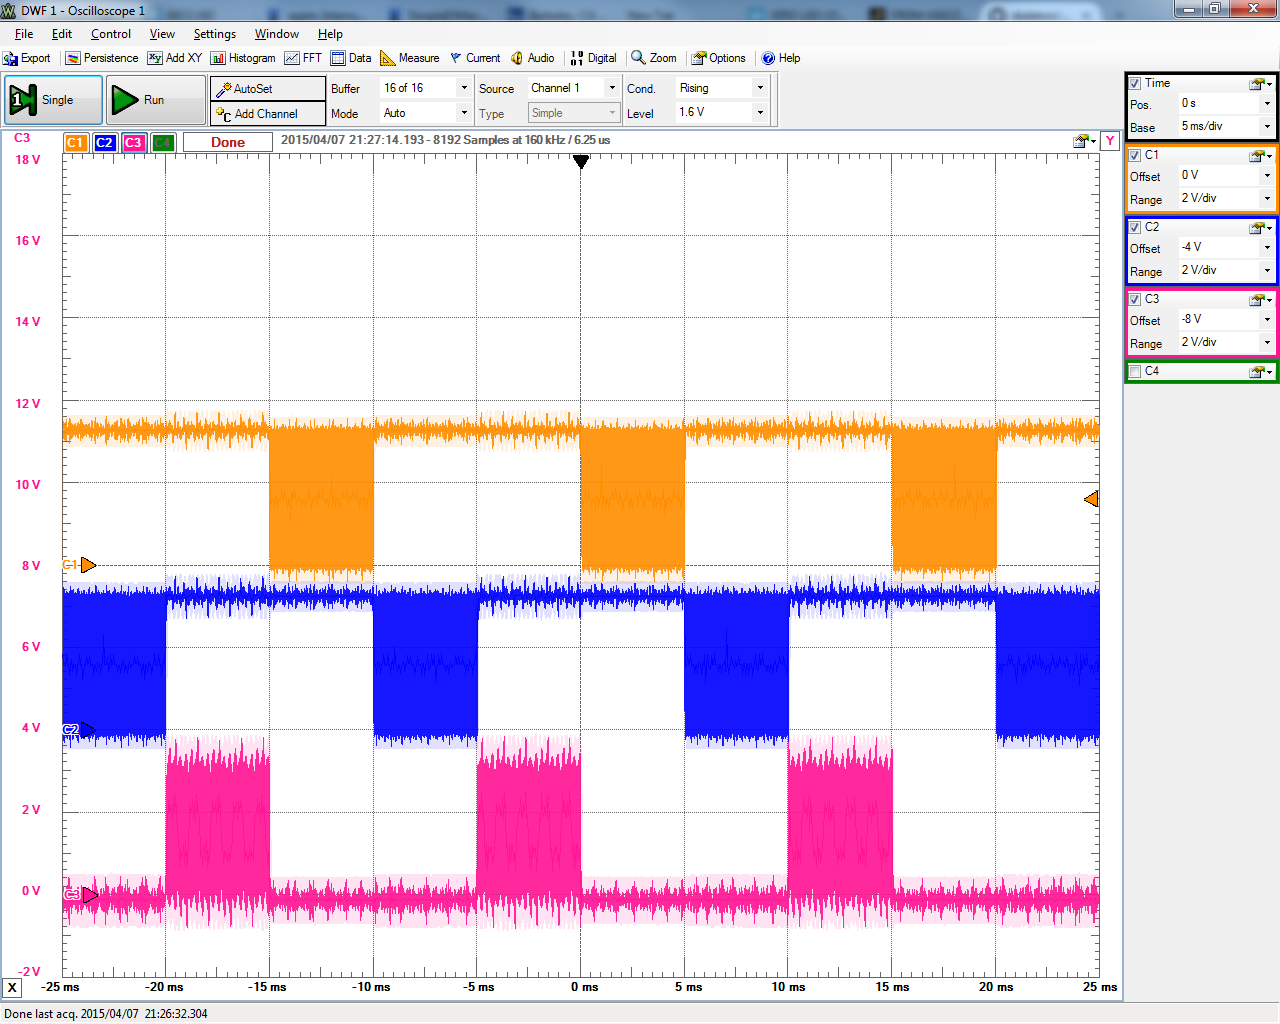
\includegraphics[width=1.0\columnwidth]{images-dis10/threading_3threads} \\
measure frequency: 5 ms/div \\
\vspace{5px}
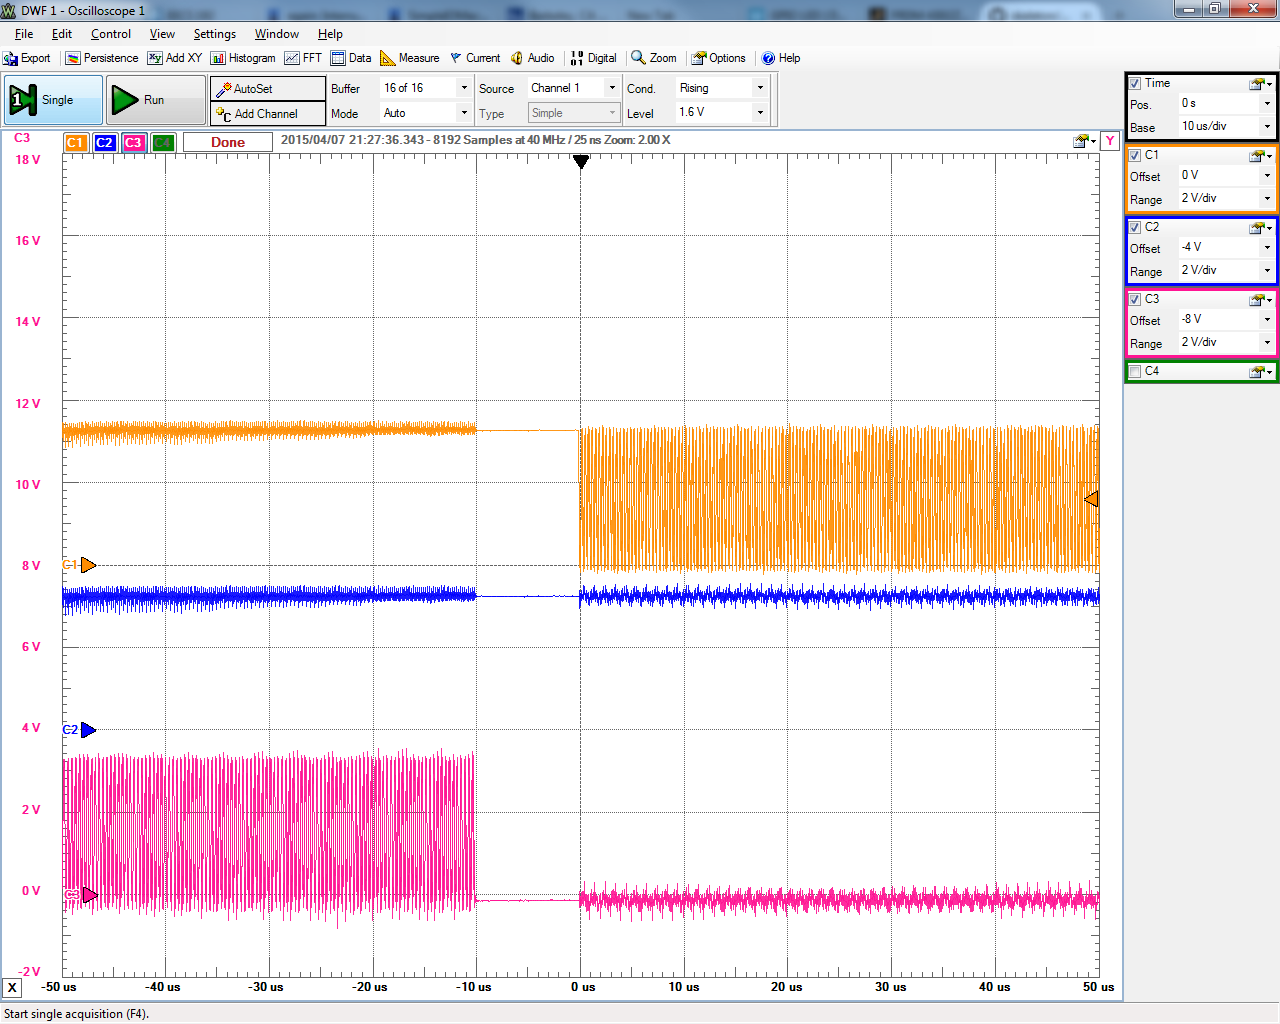
\includegraphics[width=1.0\columnwidth]{images-dis10/threading_cswitch3} \\
measure overhead: 10 us/div
}}
\end{columns}
\end{frame}

\begin{frame}[fragile]
\frametitle{Better Camera Timing}
A simple solution to meet realtime constraints is to change priorities:
\vspace{2px}
\begin{lstlisting}[language=C++,basicstyle=\ttfamily\scriptsize]
void camera_thread_fn() {
  while(1) {
    wait(CAMERA_INTEGRATION_TIME);
    Servo.set_steering(Camera.detect_line());      
  }
}
void main() {
  ...
  Thread camera_thread(camera_thread_fn);
  camera_thread.set_priority(osPriorityHigh);
  ...
}
\end{lstlisting}
\vspace{2px}
Why won't this work?
\visible<2->{
\begin{itemize}
  \item \texttt{wait} is a dumb spin loop, won't yield control to lower priority threads
  \begin{itemize}
    \item Since \texttt{camera\_thread\_fn} never sleeps, other threads ``starve''
    \item Instead, use \texttt{Thread::wait} to yield to other threads
  \end{itemize}
\end{itemize}
}
\end{frame}

\begin{frame}
\frametitle{Misc mbed RTOS topics}
\begin{columns}[t]
\column{0.646\textwidth}
\begin{itemize}
  \item \href{https://developer.mbed.org/handbook/Ticker}{Tickers} regularly calls functions using ISRs
  \begin{itemize}
    \item Standard ISR caveats apply
  \end{itemize}
  \item \href{https://developer.mbed.org/handbook/RTOS}{RtosTimer} can also regularly call functions
  \begin{itemize}
    \item All timers are handled in a single thread, \texttt{osTimerThread}
  \end{itemize}
  \item The default max number of threads is 6
  \begin{itemize}
    \item \texttt{OS\_TASKCNT} and other constants in \texttt{mbed-rtos/rtx/RTX\_Conf\_CM.c}
  \end{itemize}
\end{itemize}
\vspace{5px}
See the mbed RTOS documentation: \\
{\scriptsize\url{https://developer.mbed.org/handbook/RTOS}} \\

\column{0.323\textwidth}

\end{columns}
\end{frame}

% TODO: mention RMS / utilization guarantees somewhere?

%---------------------------------------------------------------------
\section{Software Engineering} % [?? mins]
%---------------------------------------------------------------------
\begin{frame}
\centering \huge Software Engineering
\end{frame}

%---------------------------------------------------------------------
\subsection{Abstraction}

\begin{frame}[fragile]
\frametitle{Oh Dear...}
Can you \textbf{easily} tell what this code does?
\vspace{2px}
\begin{lstlisting}[language=C++,basicstyle=\ttfamily\tiny]
// in main() loop
si = 1; si = 0;
uint16_t data[128];
for (int i=0; i<128; i++) {
  clk = 0;  clk = 1;
  data[i] = ain.read_u16();
}
uint16_t max = 0; uint8_t pos = 0;
for (int i=0; i<128; i++) {
  if (data[i] > max) {
    max = data[i]; pos = i;
  }
}
servo.write(0.075 + 0.025 * (64.0 - pos) / 64);
\end{lstlisting}
\vspace{2px}
\visible<2->{
Probably not.
}
\end{frame}

\begin{frame}[fragile]
\frametitle{Oh Dear...}
Is this better? Why?
\vspace{2px}
\begin{lstlisting}[language=C++,basicstyle=\ttfamily\tiny]
const uint8_t CAMERA_LENGTH = 128, CAMERA_HALF = CAMERA_LENGTH / 2;
void camera_read(uint16_t* data_out) {
  si = 0; si = 0;
  for (int i=0; i<CAMERA_LENGTH; i++) {
    clk = 0;  clk = 1;
    data_out[i] = ain.read_u16();
  }
}
uint8_t line_detect(uint16_t* cam_data) {
  uint16_t max = 0; uint8_t pos = 0;
  for (int i=0; i<CAMERA_LENGTH; i++) {
    if (cam_data[i] > max) {
      max = cam_data[i]; pos = i;
    }
  }
  return pos;
}
void set_steering_pct(float pct) {
  servo.write(0.075 + 0.025 * (pct));
}

// in main() loop
uint16_t cam_data[CAMERA_LENGTH];
camera_read(cam_data);
int8_t line_offset = CAMERA_HALF - line_detect(cam_data);
set_steering_pct((float)line_offset/CAMERA_HALF);
\end{lstlisting}
\end{frame}

\begin{frame}
\frametitle{Good Programming Style}
\begin{columns}[t]
\column{0.646\textwidth}
Good style produces readable and maintainable code, saving you time later
\begin{itemize}
  \item Short functions, single responsibility
  \begin{itemize}
    \item Make it easy to understand
  \end{itemize}
  \item Consistent level of abstraction
  \begin{itemize}
    \item Separate the ``what'' from the ``how''
  \end{itemize}
  \item Don't repeat yourself (DRY)
  \begin{itemize}
    \item Copypaste code is bad: making consistent changes becomes very hard
  \end{itemize}
\end{itemize}
\vspace{5px}
Want to know more? Take cs169!

\column{0.323\textwidth}

\end{columns}
\end{frame}

%---------------------------------------------------------------------
\subsection{State Machines}

\begin{frame}[fragile]
\frametitle{The Old Fashioned Way}
Here's a really basic lost line algorithm:
\vspace{2px}
\begin{lstlisting}[language=C++,basicstyle=\ttfamily\tiny]
uint16_t last_line_pos = 0;
motor.set_pwm(0.7);
while(1) {
  int16_t line_pos = line_detect(camera_data);
  if (line_pos != -1) { // line detected - follow it
    set_steering_pct(pid_update(line_pos));
  } else { // line not found - rail servo in previous direction
    if (last_line_pos < 64) {
      set_steering_pct(0.0);
    } else {
      set_steering_pct(1.0);
    }
    motor.set_pwm(0.4); // slow down
  }
  last_line_pos = line_pos;
}
\end{lstlisting}
\vspace{2px}
Is it correct?
\visible<2->{
Nope
\begin{itemize}
  \item \texttt{last\_line\_pos} immediately clobbered, but not obvious at-a-glance
  \item Implicit state in motor PWM - forget to reset motor to full speed
\end{itemize}
}
\end{frame}

\begin{frame}[fragile]
\frametitle{With State Machines}
Let's make things clearer by following the state machine model
\vspace{5px}
\begin{columns}[t]
\column{0.646\textwidth}
Write the transition function
\begin{lstlisting}[language=C++,basicstyle=\ttfamily\tiny]
enum State { FOUND, LOST_LEFT, LOST_RIGHT };

State do_transition(State current_state, int16_t line_pos, int16_t last) {
  if (current_state == FOUND) {
    if (line_pos == -1) {
      if (last <= 64) {
        return LOST_LEFT;
      } else {
        return LOST_RIGHT;
      }
    }
  } else {
    if (line_pos != -1) {
      return FOUND;
    }
  }
}
\end{lstlisting}

\column{0.323\textwidth}
\begin{figure}[h!]
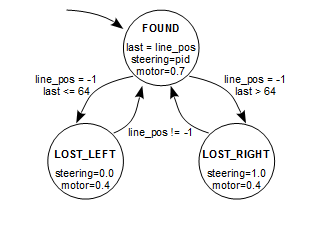
\includegraphics[width=1.0\columnwidth]{images-dis10/statemachine} \\
lost track state machine \\
graphical notation
\end{figure}
\end{columns}
\end{frame}

\begin{frame}[fragile]
\frametitle{With State Machines}
Let's make things clearer by following the state machine model
\vspace{5px}
\begin{columns}[t]
\column{0.646\textwidth}
Write the state actions
\begin{lstlisting}[language=C++,basicstyle=\ttfamily\tiny]
enum State { FOUND, LOST_LEFT, LOST_RIGHT };

void state_action(State state, int16_t line_pos, int16_t& last) {
  if (state == FOUND) {
    set_steering_pct(pid_update(line_pos));
    set_motor_pwm(0.7);
    last = line_pos;
  } else if (state == LOST_LEFT) {
    set_steering_pct(0.0);
    set_motor_pwm(0.4);
  } else if (state == LOST_RIGHT) {
    set_steering_pct(1.0);
    set_motor_pwm(0.4);
  }
}
\end{lstlisting}

\column{0.323\textwidth}
\begin{figure}[h!]
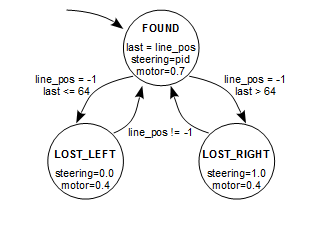
\includegraphics[width=1.0\columnwidth]{images-dis10/statemachine} \\
lost track state machine \\
graphical notation
\end{figure}
\end{columns}
\end{frame}

\begin{frame}[fragile]
\frametitle{With State Machines}
Let's make things clearer by following the state machine model
\vspace{5px}
\begin{columns}[t]
\column{0.646\textwidth}
... and put it all together
\begin{lstlisting}[language=C++,basicstyle=\ttfamily\tiny]
int16_t last = 0;
State state = FOUND;
while (1) {
  int16_t line_pos = line_detect(camera_data);
  state = do_transition(state, line_pos, last);
  state_action(state, line_pos, last);
}
\end{lstlisting}

\column{0.323\textwidth}
\begin{figure}[h!]
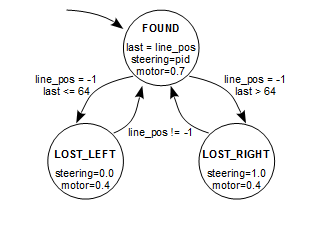
\includegraphics[width=1.0\columnwidth]{images-dis10/statemachine} \\
lost track state machine \\
graphical notation
\end{figure}
\end{columns}
\end{frame}

%---------------------------------------------------------------------
\section{Convenience vs. Performance} % [?? mins]
%---------------------------------------------------------------------
\begin{frame}
\centering \huge Convenience vs. Performance
\end{frame}

%---------------------------------------------------------------------
\subsection{Digital Output}

\begin{frame}[fragile]
\frametitle{DigitalOutput}
Given this simple block of code, guess the waveform frequency...
\vspace{2px}
\begin{lstlisting}[language=C++,basicstyle=\ttfamily\tiny]
DigitalOut wave(PTB2);
while(1) {
  wave = !wave;
}
\end{lstlisting}
\begin{columns}[T]
\column{0.45\textwidth}
\visible<2>{
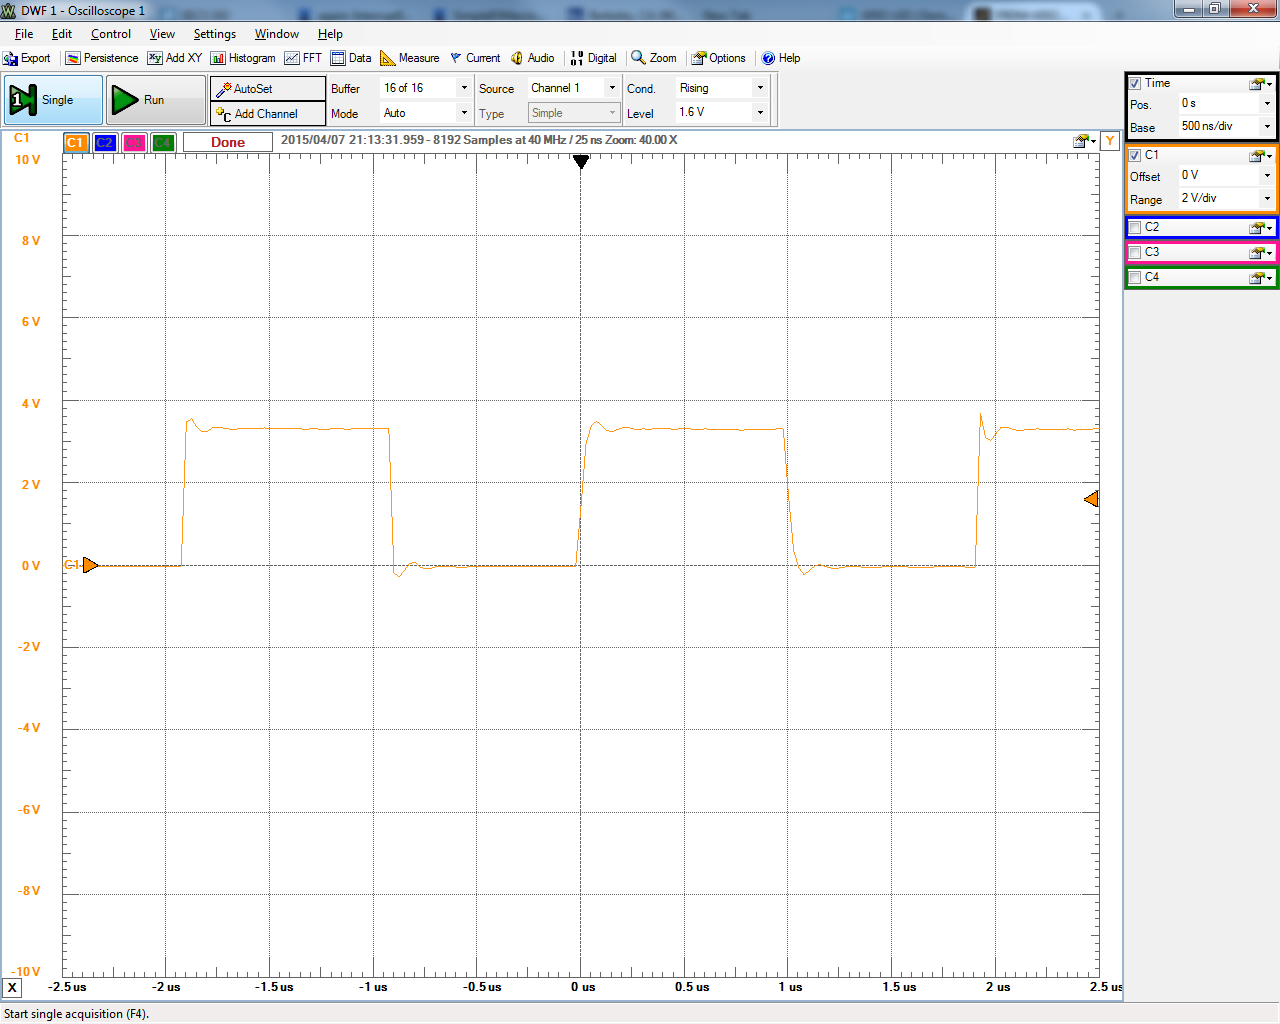
\includegraphics[width=1.0\columnwidth]{images-dis10/gpio_digitalout}
}
\column{0.45\textwidth}
\visible<2>{
About 0.5MHz! \\
(or 1 edge per us) \\
That's at least an order of magnitude slower than the instruction clock! \\
\vspace{5px}
Where might the bottleneck be?
}
\end{columns}
\end{frame}

\begin{frame}[fragile]
\frametitle{Under the Hood: How DigitalOut Works}
{\scriptsize \texttt{mbed/api/DigitalOut.h}}
\begin{lstlisting}[language=C++,basicstyle=\ttfamily\tiny]
class DigitalOut {
    void write(int value) {
        gpio_write(&gpio, value);
    }
}
\end{lstlisting}
{\scriptsize \texttt{mbed/targets/hal/TARGET\_Freescale/TARGET\_KLXX/gpio\_object.h}}
\begin{lstlisting}[language=C++,basicstyle=\ttfamily\tiny]
typedef struct {
    PinName  pin;
    uint32_t mask;
    __IO uint32_t *reg_dir;
    __IO uint32_t *reg_set;
    __IO uint32_t *reg_clr;
    __I  uint32_t *reg_in;
} gpio_t;

static inline void gpio_write(gpio_t *obj, int value) {
    if (value)
        *obj->reg_set = obj->mask;
    else
        *obj->reg_clr = obj->mask;
}
\end{lstlisting}
\vspace{5px}
Many levels of indirection for a simple register write!
\end{frame}

\begin{frame}[fragile]
\frametitle{Raw register access}
What if we skip the mbed API and directly write the register?
\vspace{2px}
\begin{lstlisting}[language=C++,basicstyle=\ttfamily\tiny]
DigitalOut wave(PTB2); // set pin as output
while(1) {
  PTB->PTOR = (0x01 << 2); // set toggle register to flip pin PTB2
}
\end{lstlisting}
\begin{columns}[T]
\column{0.45\textwidth}
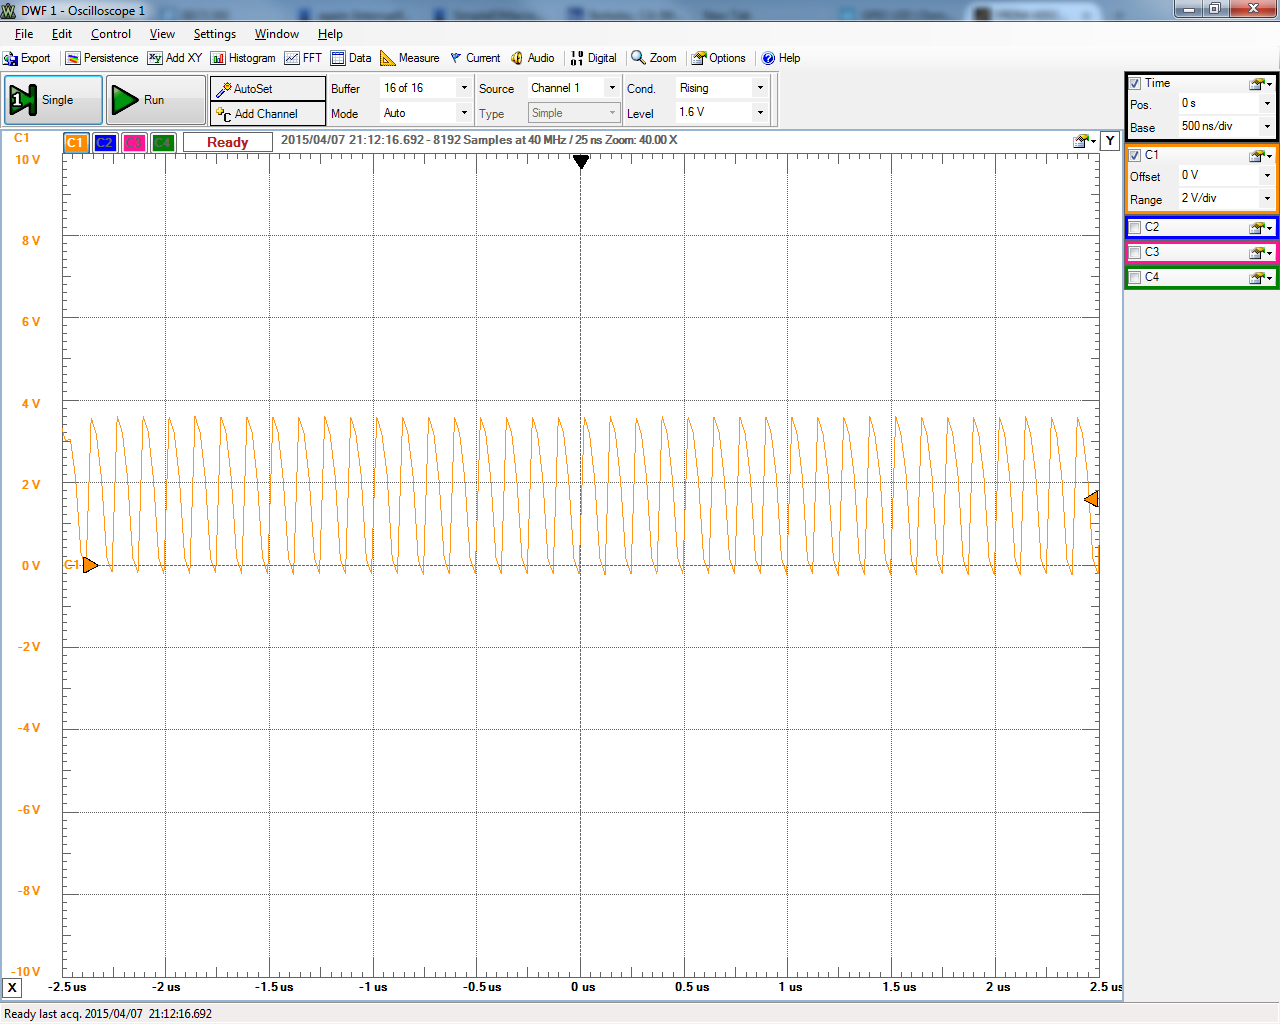
\includegraphics[width=1.0\columnwidth]{images-dis10/gpio_register_ptb_ptor}

\column{0.45\textwidth}
Much faster: about 8MHz! \\
(or 16 edges per us) \\
\vspace{10px}
{\scriptsize Each GPIO port has these registers: \\
\texttt{PDOR}: set data \\
\texttt{PSOR}: set bits \\
\texttt{PCOR}: clear bits \\
\texttt{PTOR}: toggle bits \\
\texttt{PDIR}: input \\
\texttt{PDDR}: directionality \\
See \texttt{MKL25Z4.h} for details
}
\end{columns}
\end{frame}

%---------------------------------------------------------------------
\subsection{Interrupts}

\begin{frame}[fragile]
\frametitle{InterruptIn Latency}
Similarly, let's measure the InterruptIn latency
{\tiny
\begin{itemize}
  \item ch1 (yellow) spike is ISR body
  \item ch2 (blue) toggling is main loop
  \item ch3 (pink) is interrupt signal
  \item Interrupts enabled using InterruptIn.fall(...)
\end{itemize}}
\begin{columns}[T]
\column{0.5\textwidth}
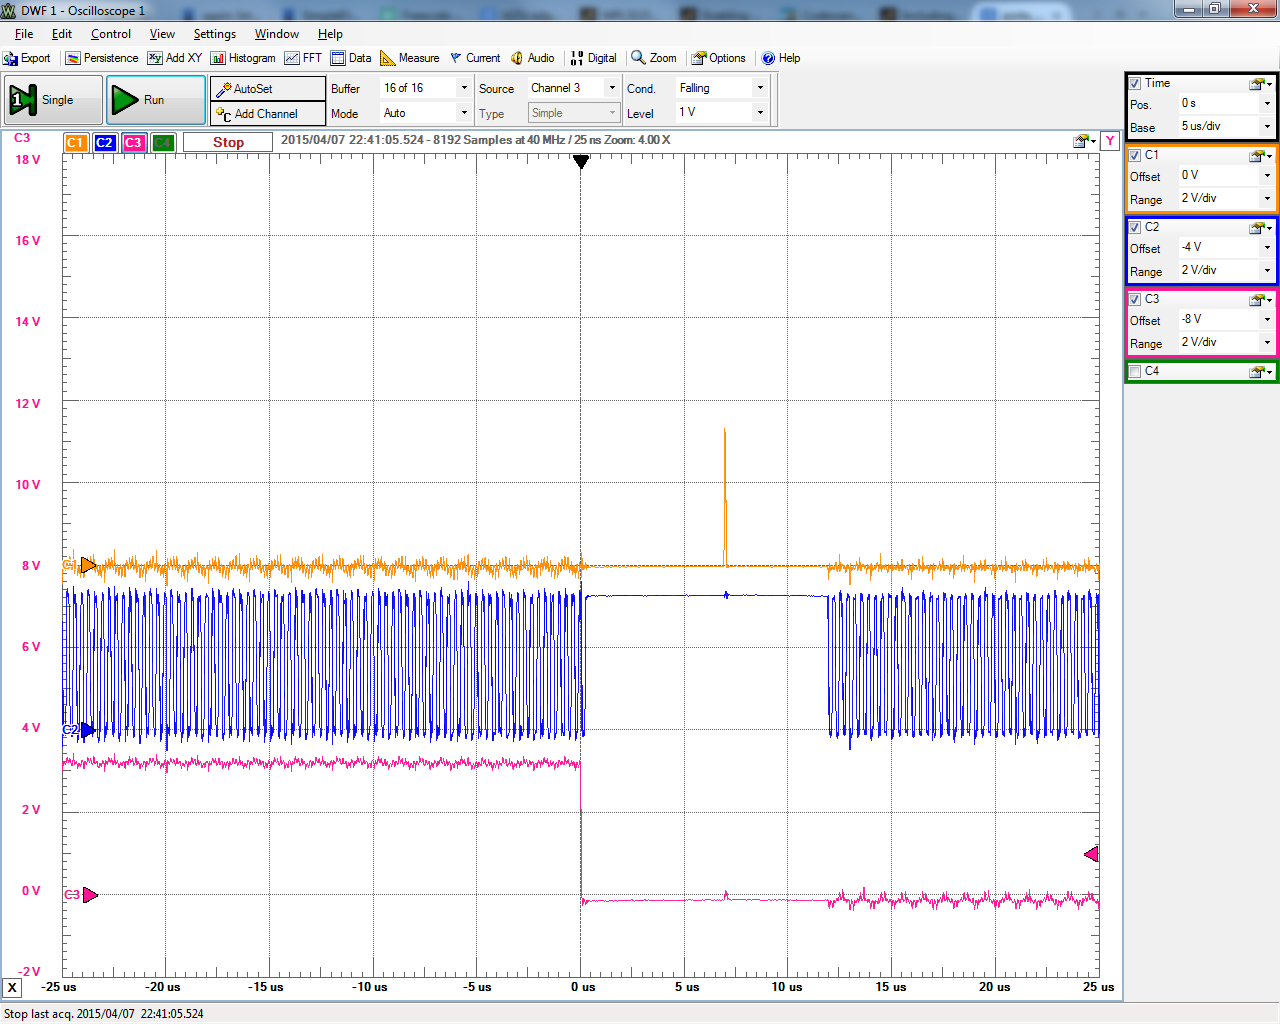
\includegraphics[width=1.0\columnwidth]{images-dis10/irq_interruptin_latency}

\column{0.4\textwidth}
About 7us from edge to interrupt \\
\end{columns}
\end{frame}

\begin{frame}[fragile]
\frametitle{InterruptIn Latency}
What about a lower level implementation?
\vspace{2px}
\begin{lstlisting}[language=C++,basicstyle=\ttfamily\tiny]
extern "C" void PORTA_IRQHandler() {
  PTB->PTOR = 0x04; PTB->PTOR = 0x04; // toggle ch1 (yellow)
  PORTA->ISFR = PORT_ISFR_ISF_MASK; // clear interrupt flags
}
NVIC_SetVector(PORTA_IRQn, (uint32_t)PORTA_IRQHandler); // set interrupt handler function
PORTA->PCR[16] = (PORTA->PCR[16] | PORT_PCR_IRQC_MASK); // enable on PTC16 / ch3 (pink)
NVIC_EnableIRQ(PORTA_IRQn);
\end{lstlisting}
\begin{columns}[T]
\column{0.5\textwidth}
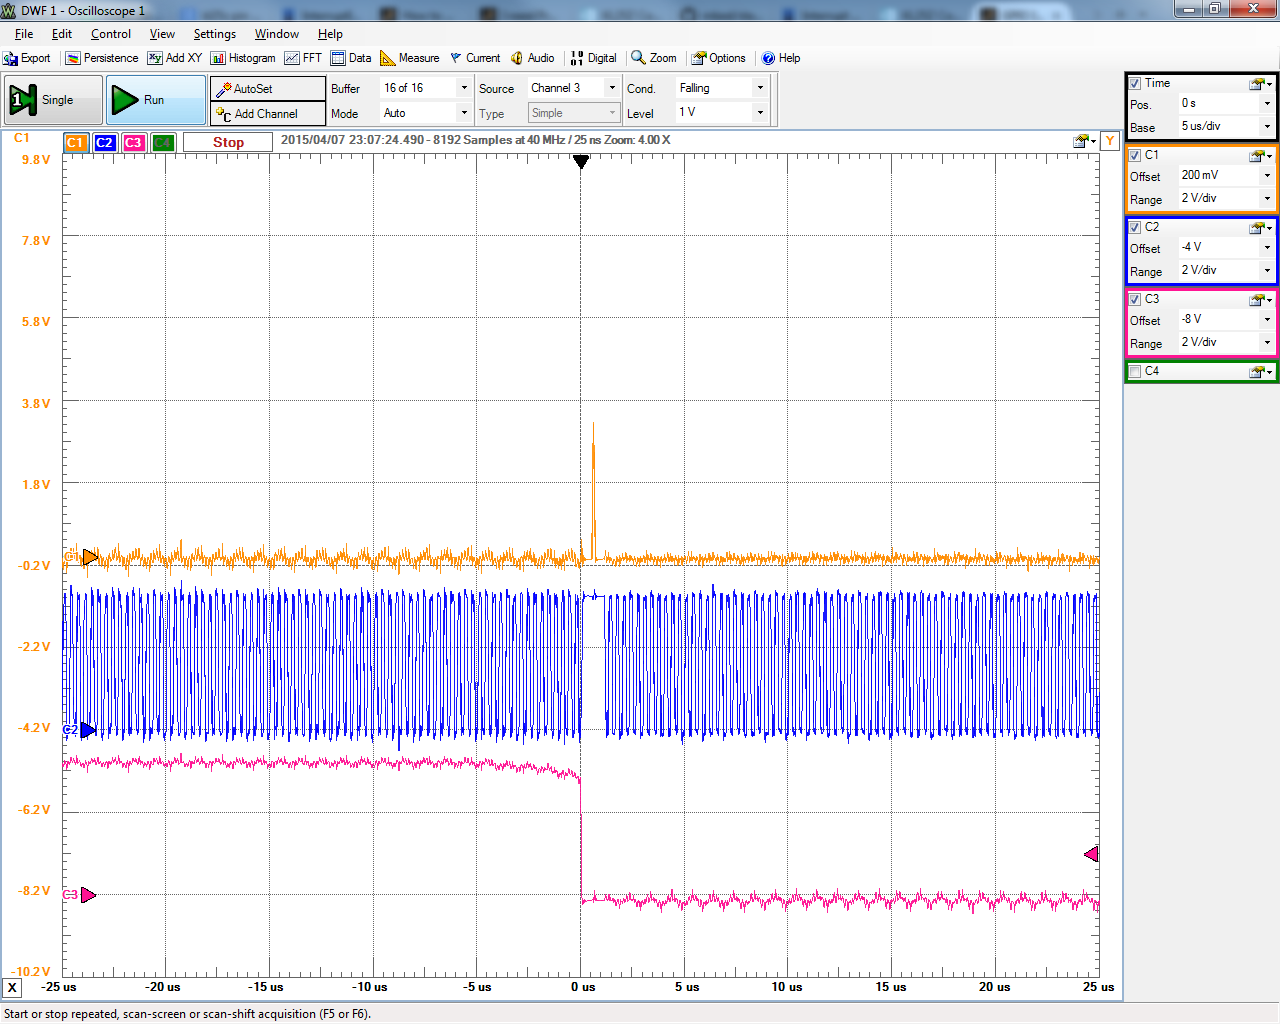
\includegraphics[width=1.0\columnwidth]{images-dis10/irq_raw_latency}

\column{0.4\textwidth}
Much faster: about 0.5us from edge to interrupt \\
\vspace{20px}
But does this really matter?
{\scriptsize
\begin{itemize}
  \item Order of magnitude faster
  \item ... but it's still microseconds
  \item Unlikely to be a bottleneck
\end{itemize}
}
\end{columns}
\end{frame}

\begin{frame}
\frametitle{Summary}
\begin{itemize}
  \item Interrupts and threading can make multitasking easier
  \begin{itemize}
    \item Also come with their set of pitfalls and issues
  \end{itemize}
  \item Write good code so you don't hate yourself later
  \item If you have high performance requirements, go below the mbed API
  \begin{itemize}
    \item But in absolute timing terms, unlikely to make a significant difference
  \end{itemize}
  \vspace{20px}
  \item Questions? Feedback?
\end{itemize}
\end{frame}

\end{document}
